\documentclass[]{article}

\usepackage[utf8]{inputenc}
\usepackage[french]{babel}           %pour un document en français
\usepackage[T1]{fontenc}

\usepackage{graphicx}                %pour insérer images et pdf entre autres

%\usepackage[left=1.5cm,right=1.5cm,top=1.5cm,bottom=1.5cm]{geometry} %réglages des marges du document
\usepackage{xcolor}
\usepackage{sectsty}
\usepackage{titlesec}
\usepackage{paralist}
\usepackage{setspace}\spacing{1.5}
\usepackage{fancyhdr}
\usepackage{lastpage}
\usepackage{dcolumn}
\usepackage{lipsum}                  %juste utile ici pour générer du faux texte
\usepackage{amsmath,amsfonts,amssymb}%extensions de l'ams pour les mathématiques American Mathematical Society 
\usepackage{hyperref}                %rend actif les liens, références croisées, toc…
%\usepackage{natbib}\bibliographystyle{agsm}
\usepackage[nottoc, numbib]{tocbibind}  
%\usepackage[shadow]
\usepackage{tikz}
\newcommand{\dsp}{Direction de la santé et de la population }

\title{bibliographie}
\author{tibaredha}
\date{March 2023}

\usepackage{Sweave}
\begin{document}
\Sconcordance{concordance:memoire.tex:memoire.Rnw:%
1 30 1 1 0 7 1 1 2 6 0 2 1 1 2 3 0 1 2 62 1}

\maketitle
%\subsectionfont{\raggedright}
%\subsubsectionfont{\raggedright}

\pagenumbering{gobble}

\begin{centering}

  \begin{center}
    \normalsize{Republique Algerienne Démocratique et Populaire}\\
    \normalsize{Ministère de Santé}\\
    \normalsize{Direction de la Santé et de la population de la Wilaya de Djelfa}\\
    \normalsize{inspection sante publique}\\
  \end{center}
  % 
  \begin{center}
    
\includegraphics[width=4cm,height=3.7cm]{img/msp.jpg}
  \end{center}
  % 
  % \begin{center}
  % \Huge{\textbf{Mémoire de Master}}\\
  % \large{Domaine : Informatique}\\
  % \textbf{}\\
  % \large{\textbf{Spécialité: Systèmes Informatiques Intelligents}}\\
  % \textbf{}\\
  % \bigskip
  % \vspace*{1cm}
  % \normalsize{\textbf{Thème}}
  % \end{center}
  % \shabox{
  % 	\begin{minipage}{0.9\textwidth}
  % 	\begin{center}
  % 	\Large{profil épidemiologique de la mortalité wilaya de djelfa}
  % 	\end{center}
  % 	\end{minipage}
  % }
  % 
  % \vspace*{1.5cm}
  % 
  % \begin{table}[h]
  %   \center
  %   \begin{tabular}{p{8cm}p{6.5cm}}
  %     \textbf{Présenté par :}   & \textbf{Proposé et dirigé par :}\\
  %       - Redha TIBA            & -	Pr. x.y \\
  %       - Azzedine BOULAOUCHE   & -	Pr. x.y\\
  %   \end{tabular}
  % \end{table}
  % 
  % \vspace*{0.5cm}
  % 
  % \begin{table}[h]
  %   \begin{tabular}{p{6.5cm}p{5cm}}
  %     \textbf{Devant le jury composé de:}&\\
  %       - \,\,\, Mme. x.y         & Présidente \\
  %       - \,\,\, Mme. x.y           & Membre \\
  %   \end{tabular}
  % \end{table}
  % 
  % 
  % \vspace*{1.7cm}
  % \begin{center}
  %   Projet N\textsuperscript{o} : 000/2023
  % \end{center}
\end{centering}








\begin{Schunk}
\begin{Sinput}
> 1 + 1
\end{Sinput}
\begin{Soutput}
[1] 2
\end{Soutput}
\begin{Sinput}
> par(mar = c(4, 4, .2, .2))
> plot(rnorm(100))
> x <- 1+1
\end{Sinput}
\end{Schunk}

You can also write inline expressions, e.g. $\pi=3.14159265358979$,
and 2 is a big number.
\LaTeX

\lipsum[1]
Lorem\footnote{Une note de bas de page.}


\tiny abcdefghijklmnopqrst\\
\scriptsize abcdefghijklmnopqrst\\
\footnotesize abcdefghijklmnopqrst\\
\small abcdefghijklmnopqrst\\
\normalsize abcdefghijklmnopqrst\\
\large abcdefghijklmnopqrst\\
\Large abcdefghijklmnopqrst\\
\LARGE abcdefghijklmnopqrst\\
\huge abcdefghijklmnopqrst\\
\Huge abcdefghijklmnopqrst\\

\normalsize


\textit Italique
\emph Texte en emphase
\textbf <U+E03A>ras
\textsc tibaredha
\underline Soffligné (à éfiiter)
\textsuperscript Effiposant
\textsubscript Indice (nécessite le package subscript)

\textcolor{red}{tibaredha}.
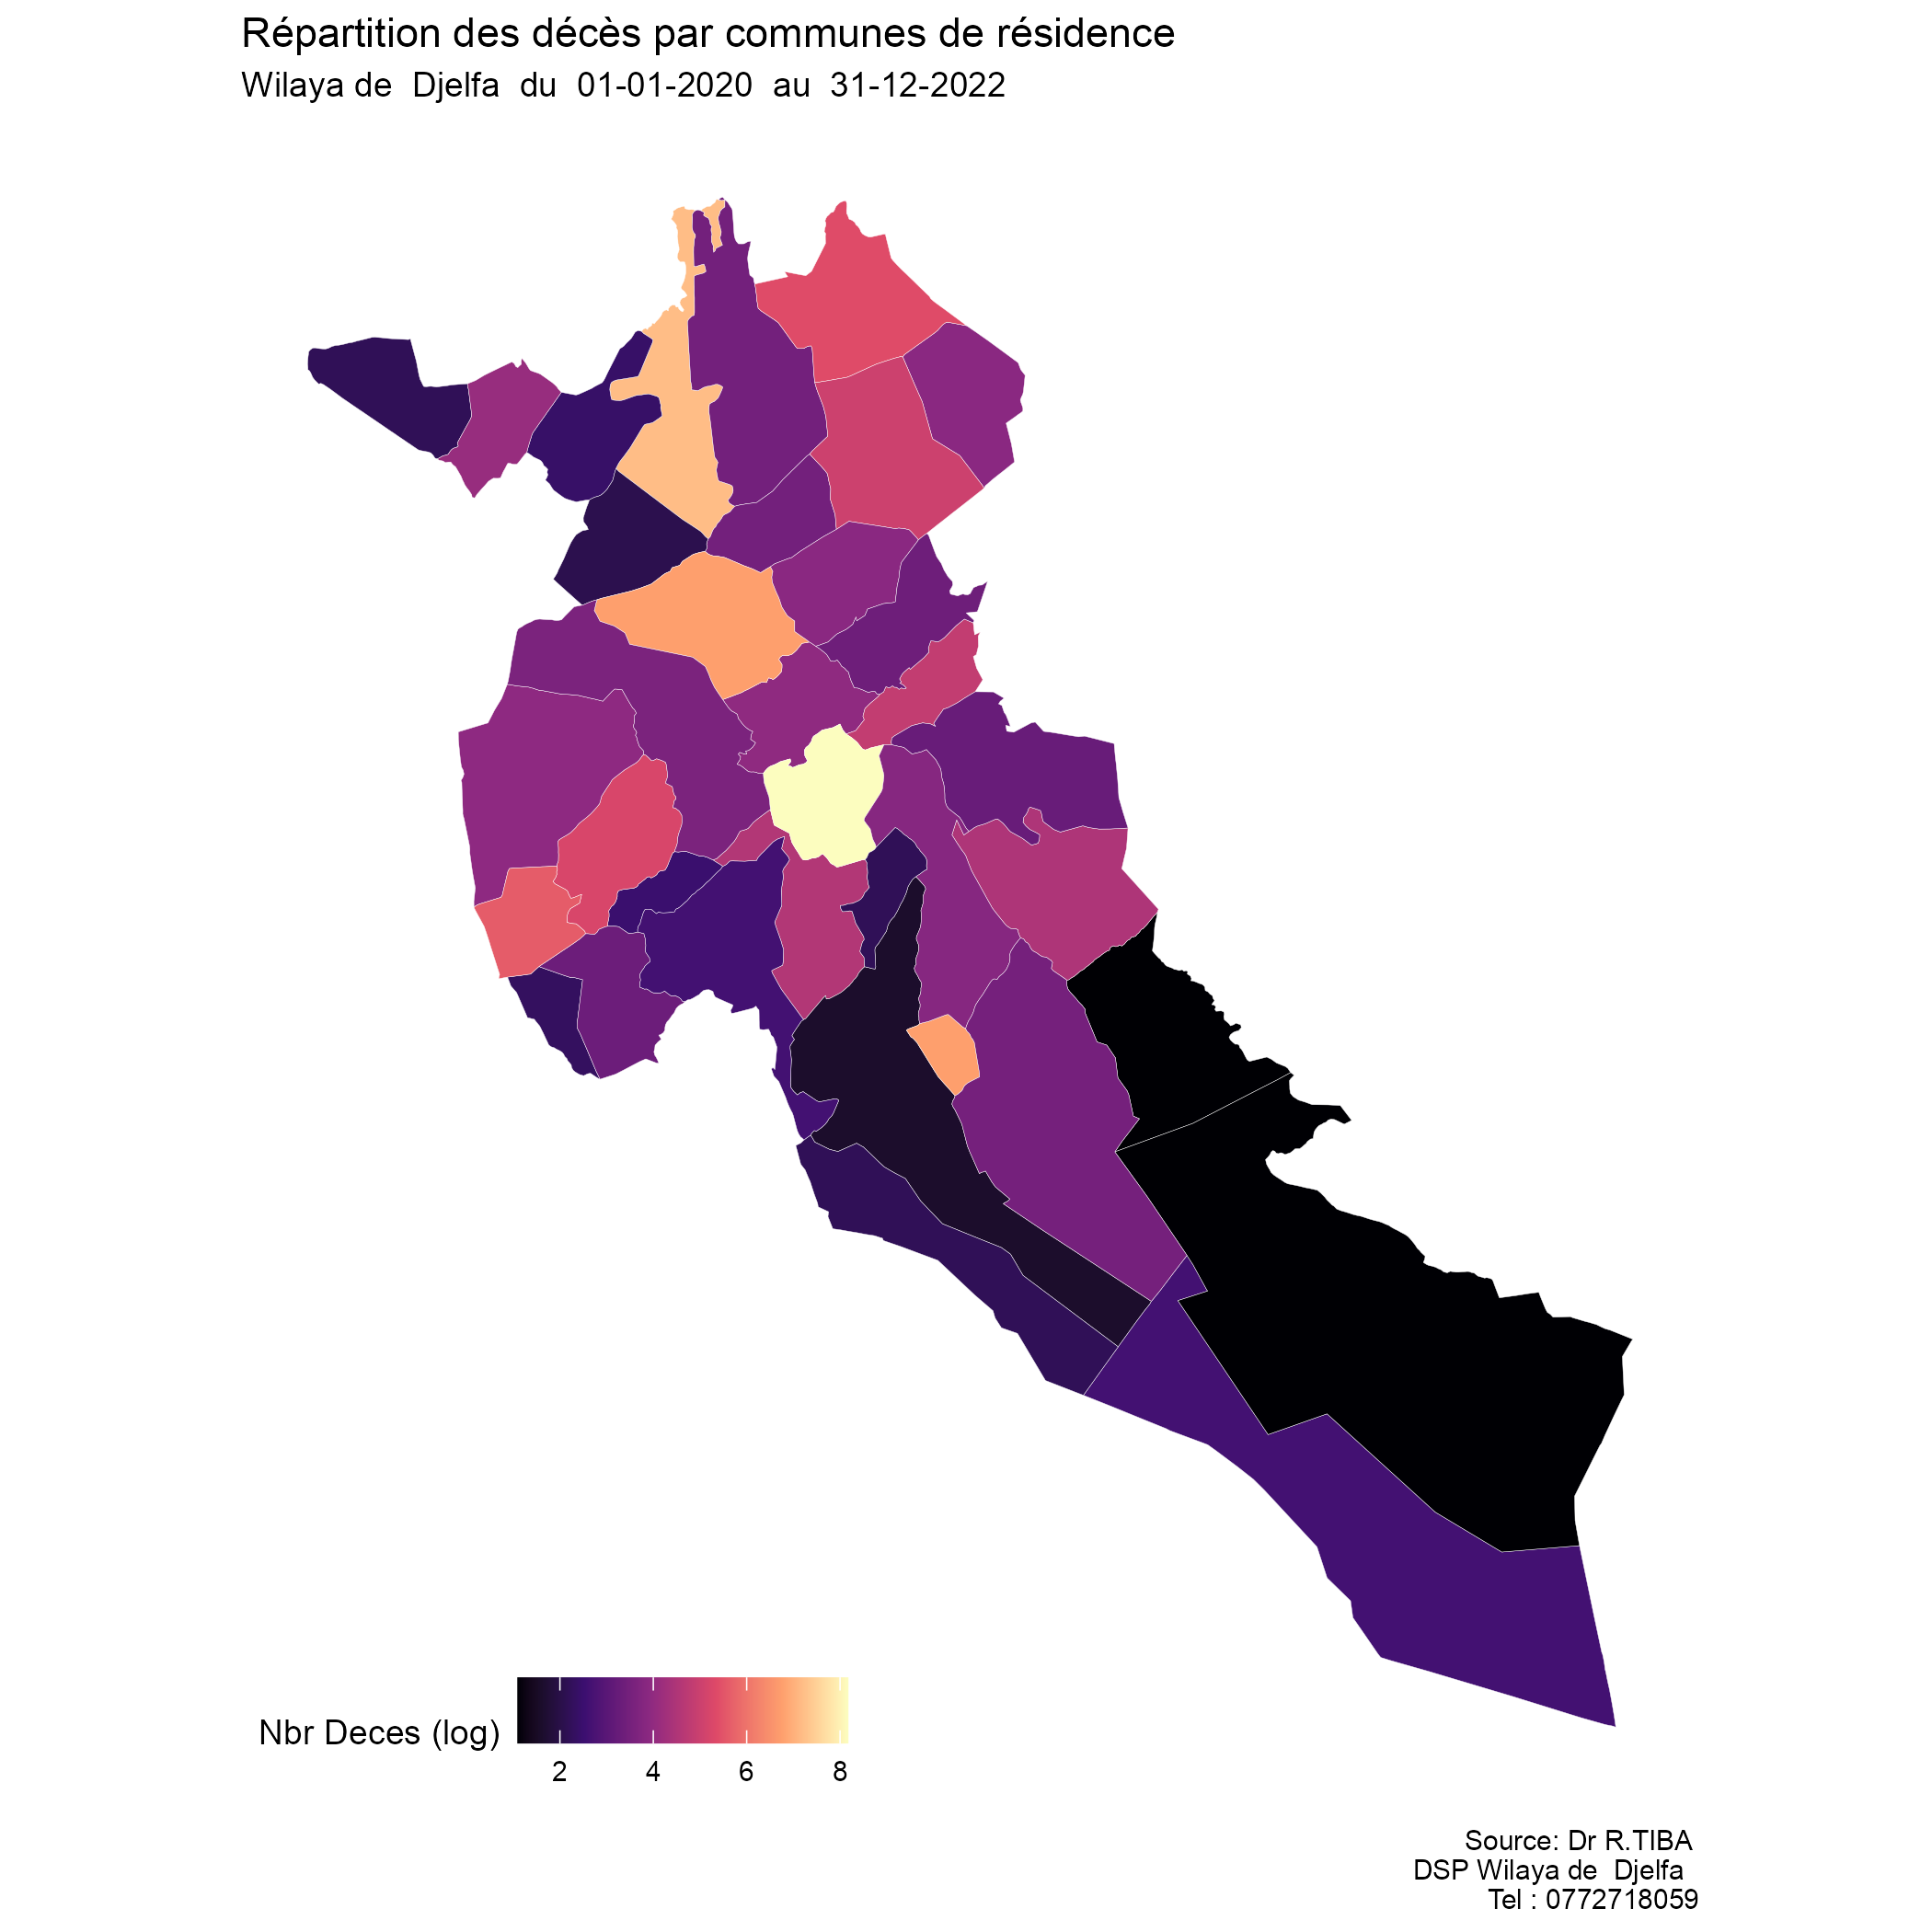
\includegraphics[]{img/SIG_commune_Djelfa}.

\begin{tabular}{|l|c|r|}
Première cellule à gauche
 & Première cellule au centre
 Première cellule à droite \\
 Seconde cellule à gauche
 & Seconde cellule au centre
 & Seconde cellule à droite \\
 \end{tabular}





%\documentclass[12pt,a4paper]{article}

\usepackage[right=2cm,left=2cm,top=2cm,bottom=2cm]{geometry}
\usepackage{luatextra}
\usepackage[french]{babel}
\usepackage{fontspec}
\setmainfont{Linux Libertine O}
\usepackage{xcolor}
\usepackage{hyperref}
	\hypersetup{
		colorlinks=true,
		linkcolor=black,
	}
\usepackage{fancyhdr}
\pagestyle{empty}

\setlength\parindent{0pt}

\begin{document}

\begin{Form}

\begin{center}
	\textbf{\uppercase{Attestation de déplacement dérogatoire}} \\
	En application de l'article 3 du décret du 23 mars 2020 prescrivant les mesures générales
	nécessaires pour faire face à l'épidémie de Covid19 dans le cadre de l'état d'urgence sanitaire 
\end{center}

Je soussigné(e), \\

\TextField[width=5cm,borderwidth=0pt]{Mme/M. :} \\
\TextField[width=5cm,borderwidth=0pt]{Né(e) le :} \\
\TextField[width=5cm,borderwidth=0pt]{À :} \\
\TextField[width=14cm,borderwidth=0pt]{Demeurant :} \\

certifie que mon déplacement est lié au motif suivant (cocher la case) autorisé par l'article 3
du décret du 23 mars 2020 prescrivant les mesures générales nécessaires pour faire face à
l'épidémie de Covid19 dans le cadre de l'état d'urgence sanitaire\footnote{Les personnes
souhaitant bénéficier de l'une de ces exceptions doivent se munir s'il y a lieu, lors de leurs
déplacements hors de leur domicile, d'un document leur permettant de justifier que le déplacement
considéré entre dans le champ de l'une de ces exceptions.} :\\

\begin{minipage}{0.1\textwidth}
	\CheckBox[bordercolor=black]{}
\end{minipage}
\begin{minipage}{0.89\textwidth}
	Déplacements entre le domicile et le lieu d'exercice de l'activité professionnelle,
	lorsqu'ils sont indispensables à l'exercice d'activités ne pouvant être organisées sous
	forme de télétravail ou déplacements professionnels ne pouvant être différés\footnotemark.
\end{minipage}
\footnotetext{À utiliser par les travailleurs non-salariés, lorsqu'ils ne peuvent disposer d'un 
	justificatif de déplacement établi par leur employeur.}

\vspace{5mm}

\begin{minipage}{0.1\textwidth}
	\CheckBox[bordercolor=black]{}
\end{minipage}
\begin{minipage}{0.89\textwidth}
	Déplacements pour effectuer des achats de fournitures nécessaires à l’activité
	professionnelle et des achats de première nécessité\footnotemark{} dans des établissements dont les
	activités demeurent autorisées (liste sur gouvernement.fr).
\end{minipage}
\footnotetext{Y compris les acquisitions à titre gratuit (distribution de denrées alimentaires\dots) et
	les déplacements liés à la perception de prestations sociales et au retrait d'espèces.}
	
\vspace{5mm}

\begin{minipage}{0.1\textwidth}
	\CheckBox[bordercolor=black]{}
\end{minipage}
\begin{minipage}{0.89\textwidth}
	Consultations et soins ne pouvant être assurés à distance et ne pouvant être différés ;
	consultations et soins des patients atteints d'une affection de longue durée.
\end{minipage}

\vspace{5mm}

\begin{minipage}{0.1\textwidth}
	\CheckBox[bordercolor=black]{}
\end{minipage}
\begin{minipage}{0.89\textwidth}
	Déplacements pour motif familial impérieux, pour l'assistance aux personnes
	vulnérables ou la garde d’enfants.
\end{minipage}

\vspace{5mm}

\begin{minipage}{0.1\textwidth}
	\CheckBox[bordercolor=black]{}
\end{minipage}
\begin{minipage}{0.89\textwidth}
	Déplacements brefs, dans la limite d'une heure quotidienne et dans un rayon maximal
	d'un kilomètre autour du domicile, liés soit à l'activité physique individuelle des
	personnes, à l'exclusion de toute pratique sportive collective et de toute proximité avec
	d'autres personnes, soit à la promenade avec les seules personnes regroupées dans un
	même domicile, soit aux besoins des animaux de compagnie.
\end{minipage}

\vspace{5mm}

\begin{minipage}{0.1\textwidth}
	\CheckBox[bordercolor=black]{}
\end{minipage}
\begin{minipage}{0.89\textwidth}
	Convocation judiciaire ou administrative.
\end{minipage}

\vspace{5mm}

\begin{minipage}{0.1\textwidth}
	\CheckBox[bordercolor=black]{}
\end{minipage}
\begin{minipage}{0.89\textwidth}
	Participation à des missions d'intérêt général sur demande de l'autorité administrative.
\end{minipage} \\

\TextField[width=8cm,borderwidth=0pt]{Fait à :} \\
\TextField[width=4cm,borderwidth=0pt]{Le :} 
\TextField[width=1cm,borderwidth=0pt,maxlen=2]{à} 
\TextField[width=1cm,borderwidth=0pt,maxlen=2]{h} \\
(Date et heure de début de sortie à mentionner obligatoirement) \\

\TextField[width=14cm,borderwidth=0pt]{Signature :} 

\end{Form}

\end{document}



%
\section{abstaract}
Dans le cadre du système d’information actif mis
en place par le service d’épidémiologie sur la mortalité
hospitalière au CHU de Blida (Algérie), une étude a été
réalisée pour apprécier l’importance et l’évolution de la
mortalité néonatale enregistrée au CHU au cours des années
1999-2006, ainsi que celles des causes du décès néonatal.\\
La Classification internationale des maladies (CIM-9) a
été utilisée pour coder la nature de la maladie causale. Les
opérations de saisie, de contrôle et d’analyse ont été effectuées
par l’utilisation du logiciel ÉpiInfo™dans sa sixième version.
Au total, 2 167 décès néonatals ont été enregistrés au CHU
pendant la période d’étude, soit une mortalité proportionnelle
de 25,4 \%. La mortalité néonatale précoce (0-6 jours) a
représenté 83,4 \% de l’ensemble de la mortalité néonatale.
Près des deux tiers des décès néonatals précoces sont
intervenus dans les trois premiers jours de vie. L’évolution
mensuelle du nombre de décès néonatals précoces a dessiné
une tendance significativement à la hausse au cours de la
période d’étude (p < 0,05) sans mise en évidence d’effet
saisonnier. Le rapport de masculinité était pratiquement le
même pour la mortalité néonatale précoce et tardive, respectivement
1,4 et 1,5. La prématurité a représenté 42,1 \% des
causes de décès de lamortalité néonatale précoce, suivie par le
syndrome de détresse respiratoire et les infections ; respectivement
17 et 14,4 \%. Les infections ont représenté, avec une
fréquence relative de 36,2 \%, la cause la plus fréquente pour
la mortalité néonatale tardive. Le taux de mortalité néonatale
précoce au cours de la période d’étude, lorsque celui-ci admet
pour dénominateur le nombre de nouveau-nés admis en
néonatalogie pour exprimer la mortalité de service, était de
15,6 \%. Pendant toute la période d’étude, le taux de mortalité
néonatale précoce, en déduisant les décès survenus parmi
les nouveau-nés transférés, pouvait être estimé à 19,2 pour
1 000 naissances vivantes, tandis que le taux de mortalité
néonatale globale pouvait être estimé à 22,3 pour 1 000 naissances
vivantes. Aucune tendance temporelle significative n’a
été mise en exergue. Le CHU de Blida ne se caractérise pas par
un risque inférieur de mortalité néonatale par rapport à celui
enregistré à l’échelle nationale. Les données du CHU de Blida
contribuent à mesurer le degré d’atteinte d’objectifs fixés par
le Programme national sur la périnatalité.
%\input{./memoire/introduction}
%\input{./memoire/materiel_et_methodes}
%\input{./memoire/resultat}
%La mortalité néonatale a donc constitué un quart des décès
survenant au CHU de Blida pendant la période d’étude. Une
MP de cet ordre (28 %) a été retrouvée au CHU d’Annaba
(Algérie) au début de la décennie écoulée [8]. Il est frustrant
de ne pouvoir pousser plus loin les comparaisons, car les
tentatives visant à établir des statistiques de mortalité et de
morbidité avec des méthodes standardisées sont restées très
limitées, même à l’échelle des CHU [7].
Les décès néonatals survenus en dehors du service de
néonatalogie ont constitué moins de 4 % (3,3 %) de
l’ensemble des décès néonatals survenus au CHU. Du fait
de cette faible proportion, ces décès ont été comptabilisés
avec ceux qui sont survenus en néonatalogie pour calculer
la mortalité de service et pour déterminer les autres taux de
mortalité néonatale.
La mortalité néonatale précoce a représenté plus de 80 %
de la mortalité néonatale au CHU de Blida : elle semblait du
même ordre de grandeur que celle enregistrée dans la plupart
des pays de la sous-région ouest africaine où elle pouvait
constituer 75 à 90 % de la mortalité néonatale [2,10]. Le
risque mesurant la mortalité de service était aussi identique à
celui enregistré dans un hôpital de Côte-d’Ivoire [19].
Les comparaisons, malgré les difficultés reconnues
qu’elles suscitent du point de vue de la validité des données
et de la standardisation des définitions [11], sont encore plus
intéressantes lorsque le taux de mortalité néonatale admet
comme dénominateur le nombre de naissances vivantes
enregistré dans l’établissement.
Le taux moyen de mortalité néonatale précoce à l’hôpital
de gynécologie-obstétrique de Hanoi pendant la période
1991-1995, de l’ordre de 24 pour 1 000 naissances vivantes
[13], était approximativement identique à celui enregistré au
CHU de Blida. Au CHU de Dakar, pendant la décennie
1994-2003, ce taux était encore plus élevé : 45,5 pour
1 000 et augmentait même à 67,5 pour 1 000 lorsqu’il était

tenu compte des nouveau-nés transférés des maternités
périphériques et dont la proportion représentait 4,2 % [9].
Le taux de mortalité néonatale précoce à l’hôpital de
gynécologie-obstétrique de Hanoi n’était plus, en 1995, que
de 15,3 pour 1 000, chute essentiellement due à une
augmentation de la proportion d’accouchements normaux
et à une diminution drastique de la proportion des cas
adressés par les maternités périphériques, suite à un
changement dans la politique nationale de santé intervenu
en 1992 [13]. Ce taux restait néanmoins élevé lorsqu’il était
comparé à celui enregistré en 1991 dans un hôpital
universitaire de Malaisie : 5,5 pour 1 000 naissances
vivantes [3]. Une baisse du taux de mortalité néonatale a
aussi été enregistrée dans un hôpital universitaire nigérian, de
50 pour 1 000 en 1974 à 16 pour 1 000 en 1981, baisse
expliquée par une réduction de la mortalité chez les enfants
dont le poids de naissance dépassait 2 500 g et ceux
souffrant d’asphyxie [21]. Le taux de mortalité néonatale
précoce a atteint 34 pour 1 000 dans un centre universitaire
de Madagascar [5].
Le taux de mortalité néonatale précoce pouvait être
cependant bas en Afrique, de l’ordre de 14 pour 1 000 dans
un district sanitaire au Burkina Faso, tandis que le taux de
mortalité néonatale globale était de 24 pour 1 000 [25].
Le taux de mortalité néonatale précoce dans un district
rural au Mali était aussi faible (17 pour 1 000), tandis que le
taux de mortalité néonatale tardive était de 7 pour 1 000, soit
un taux de mortalité néonatale globale de 24 pour 1 000, plus
faible que le taux national estimé à 57 pour 1 000 [24].
Des taux nationaux du même ordre de grandeur pouvaient
être retrouvés pour l’Afrique et l’Asie. Pour l’Afrique au sud
du Sahara, le taux moyen régional en 1995 était estimé à
39 pour 1 000 (variant de 13 pour 1 000 au Kenya à 108 pour
1 000 au Sénégal), tandis que pour l’Asie du Sud, pour la
même année, le taux de mortalité néonatale variait de 42 à
57 pour 1 000 [14].
Le taux de mortalité néonatale précoce, à partir des
données portant sur 7 993 grossesses dans six pays en
développement, pouvait encore être plus faible : 9 pour
1 000 naissances vivantes [20]. Au Québec, pendant la
période 1976-2005, le taux de mortalité néonatale précoce
n’a été que de 2,9 pour 1 000, alors que le taux de mortalité
néonatale global était de 3,4 pour 1 000 [15]. En République
tchèque, au milieu des années 1990, le taux de mortalité
néonatale global n’était plus que de 3,8 pour 1 000 [16].
On peut à ce niveau mettre en exergue que le CHU de
Blida ne se distingue finalement pas par un risque moins
élevé de mortalité néonatale, puisqu’il enregistre des taux
similaires à ceux enregistrés au niveau national [18]. Par
ailleurs, le risque annuel de décéder pour un nouveau-né,
exprimé pour 1 000 naissances vivantes, est resté stationnaire
pendant toute la période d’étude, malgré la tendance à la
baisse enregistrée pour la mortalité correspondante de

service. Il est vrai que la proportion des nouveau-nés
transférés des maternités périphériques était relativement
élevée ; un nouveau-né sur cinq. Cependant, la proportion
annuelle de ces transférés a même dessiné une tendance à la
baisse (r0 = –0,88, p = 0,01), passant de 30,1 % en 2000
(proportion la plus élevée enregistrée) à 17,5 % en 2006
(proportion la plus basse enregistrée), suggérant que la
fonction de centre de référence des grossesses à risque pour
la région dévolue au CHU n’a pas été accrue au cours de
la période d’étude. De fait, cette période n’a été caractérisée
ni par l’acquisition de nouveaux équipements, ni par la mise
en place de nouvelles techniques d’exploration ou de soins,
à l’exception d’efforts consentis en matière d’hygiène
hospitalière.
La surmortalité masculine en matière de décès néonatals
est constatée dans presque toutes les recherches antérieures,
avec un sex-ratio par exemple de 1,3 pour les décès précoces
dans un centre hospitalier universitaire malgache [5], et a été
aussi retrouvée au Maroc [1].
Parmi les causes de mortalité néonatale précoce identifiées
à travers le monde, la prématurité est souvent retrouvée en
première position. Il est possible, dans notre série, que
quelques faux cas de prématurité aient été inclus, notamment
des hypotrophiques à terme d’un poids de naissance inférieur
à 2 500 g (date des dernières règles inconnue ou douteuse,
absence de contrôle par une échographie précoce et nondétermination
à la naissance de l’âge gestationnel par la
morphologie et l’examen neurologique). Malgré ces réserves,
on peut considérer que la prématurité a représenté
pendant la période d’étude plus de 40 % des décès néonatals
précoces. Une proportion supérieure à 70 % a été retrouvée
à l’hôpital de gynécologie-obstétrique de Hanoi [13] et au
CHU de Lomé, au Togo, au début des années 1990 [4]. Une
proportion de l’ordre de 50 % a été retrouvée à l’institut de
nutrition et de santé en Guinée [10].
Il semble bien que la prématurité puisse représenter plus
de 60 % des causes de décès néonatals précoces [20].
Cependant, cette contribution peut être plus faible : de
l’ordre de 23 % dans un district sanitaire au Burkina
Faso [25].
La prématurité a souvent été décrite comme une * maladie
à caractère social très prononcé *, car la prématurité est plus
fréquente parmi les enfants de femmes pauvres et peu
éduquées [13]. Le taux de prématurité (naissance avant
37 semaines de gestation), qui varierait de 5 à 9 % dans les
pays en développement [23], reste en réalité du même ordre
de grandeur dans les pays développés et dépasserait 12 %
aux États-Unis [12].
La fréquence de la prématurité reste aussi élevée et ne
semble pas baisser, malgré les avancées réalisées dans la
connaissance des facteurs de risque et l’introduction de
mesures médicales pour lutter contre ce problème de santé
publique. Cependant, des progrès considérables ont été


enregistrés en matière de survie des nouveau-nés prématurés
[12,17].
La proportion des prématurés décédés parmi les nouveaunés
pourrait être estimée à environ 1 % dans notre série
(844-78 979), mais la létalité due à la prématurité ne peut être
estimée, étant donné que le nombre total des prématurés nés
au CHU n’a pu être établi. La mortalité élevée chez les
prématurés est due au fait que les nouveau-nés prématurés
sont très vulnérables aux risques d’asphyxie et d’infection
par immaturité des fonctions immunitaire, respiratoire, etc.
L’infection a aussi été identifiée comme une cause
majeure de mortalité néonatale, dépassant la contribution
de la prématurité, et pouvant représenter jusqu’à 50 % des
causes de la mortalité néonatale [25]. Dans ce district
sanitaire, l’infection a représenté la première cause de
mortalité pendant les deux phases de la période néonatale,
mais était plus impliquée, comme au CHU de Blida, dans des
proportions différentes il est vrai, dans la phase tardive que
dans la phase précoce. Dans notre série, les infections
nosocomiales ont probablement constitué l’essentiel des
infections en surpassant le poids des infections d’origine
maternofoetale, mais le problème n’a pu être quantifié. Les
efforts consentis en matière d’hygiène hospitalière pourraient
expliquer les pourcentages relativement bas enregistrés en
2006, concernant la contribution des infections dans la
survenue de décès néonatals.
Les malformations congénitales ont constitué 11,1 % de
l’ensemble des décès néonatals. Nonobstant les nouveau-nés
transférés des maternités périphériques et qui seraient
atteints d’anomalies congénitales, les malformations n’ont
constitué que 0,3 % des naissances vivantes. Le même taux
a été retrouvé à l’hôpital de gynécologie-obstétrique de
Hanoi [13], mais ces taux sont probablement sous-estimés,
car le diagnostic est clinique, et les malformations mineures
ne sont pas rapportées. Il est parfois reconnu, parmi les
décès néonatals précoces, qu’un nouveau-né sur deux
décède dans les premières 24 heures de vie [18,13]. À
Blida, cette proportion était de 25 % environ, mais dépassait
55 % lorsqu’elle était mesurée dans les 48 premières
heures de vie.
Tous les décès néonatals ne sont certainement pas
évitables. Mais la moitié d’entre eux pourraient être évités
grâce à des mesures simples et peu coûteuses. Des pays
comme la Colombie ou le Sri Lanka qui enregistrent moins
de 15 décès pour 1 000 naissances vivantes ont fait la preuve
que des techniques coûteuses ne sont pas un préalable à une
réussite en la matière. Dans la plupart des pays, la mortalité
des enfants dont la mère a bénéficié de soins prénatals et de
soins qualifiés à l’accouchement est généralement inférieure
de plus de la moitié à la mortalité des enfants dont la mère n’a
pas bénéficié de ce type de soins, même si le problème de
la fragmentation actuelle des soins au nouveau-né reste
posé [22].
	
%\section{conclusion}
L’Algérie a pris conscience du lourd fardeau représenté par la
mortalité néonatale en mettant en place un Programme
triennal national sur la périnatalité. La surveillance de la
grossesse et du travail, d’une part, et la prise en charge
immédiate du nouveau-né par une équipe obstétricopédiatrique,
d’autre part, sont les deux piliers de ce programme,
dont des objectifs quantifiés concernent, par exemple, une
réduction de 25 \% de la mortalité néonatale précoce et une
réduction de 30 \% de la mortalité des nouveau-nés de faible
poids de naissance d’ici 2009 [18].
Les données du CHU de Blida sur la mortalité néonatale,
décrivant une période fort homogène, devraient contribuer
à mesurer le degré d’atteinte d’objectifs fixés de ce
programme, d’autant plus que le risque de mortalité
néonatale déterminé pour le CHU rejoint celui enregistré à
l’échelle nationale.
Conflit d’intérêt : aucun.	
%\input{./memoire/références}


\bibliography{bibliography/bib}
\bibliographystyle{plain}
\end{document}
